% -*- latex -*- This is a LaTeX document.
% $Id: oopsla02.tex,v 1.32 2002-11-15 21:12:17 cananian Exp $
%%%%%%%%%%%%%%%%%%%%%%%%%%%%%%%%%%%%%%%%
%\documentclass[preprint]{acmconf}
\documentclass{acmconf}
% don't forget to turn off 'preprint' before submission!
%\usepackage[section,plain]{algorithm}
%\usepackage{amsthm} % proof environment
%\usepackage{amstext} % the \text command for math mode (replaces \mbox)
\usepackage{varioref} % \vref command
\usepackage{graphicx} % for eps figures
\usepackage{color}
\usepackage{comdef}
\newcommand{\figscale}{1.0}

%setup varioref package
\renewcommand{\reftextbefore}{on the preceding page}\vrefwarning

\newcommand{\mycomment}[1]{}
\newcommand{\meet}{\ensuremath{\sqcap}}

\renewcommand{\floatpagefraction}{0.8}
\newcommand{\topfigrule}{\vspace*{9.6pt}%
  \rule{0.88\columnwidth}{0.4pt}\vspace{-10pt} }

\title{\bf Data Size Optimizations for Java Programs}

\author{C.~Scott~Ananian and Martin~Rinard\\
        Laboratory for Computer Science\\
        Massachusetts Institute of Technology\\ 
        Cambridge, MA 02139 \\ 
        {\tt \{cananian, rinard\}@lcs.mit.edu} }

\begin{document}
% in preprint mode, tag pages with a revision identifier.
%\pagestyle{myheadings}\markboth{$ $Revision: 1.32 $ $}{$ $Revision: 1.32 $ $}
\bibliographystyle{plain}

\maketitle

% abstract
\begin{abstract}
We present a set of techniques for reducing the memory consumption of
object-oriented programs. These techniques 
include optimizations that eliminate fields with
constant values, reduce the sizes of fields based on the range
of values that can appear in each field, and use a variety of
transformations to eliminate fields with common default values
or usage patterns from the majority of objects that originally
contained these fields. We can apply these optimizations both 
to fields declared by the programmer and to implicit fields in
the runtime object header. We use a variety of program analysis 
algorithms to extract the information required to apply these
optimizations. 

We have implemented these techniques in the MIT FLEX compiler
system and applied them to the programs in the SPECjvm98 
benchmark suite. Our experimental results show that 
our combined techniques can significantly reduce the amount
of memory required to store the objects in our benchmark
suite.  Some of the optimizations reduce the overall execution time;
others may impose modest performance penalties.

\end{abstract}

\section{Introduction}

This paper presents a set of techniques for reducing the
amount of data space required to represent objects
in object-oriented programs. Our techniques optimize
the representation of both the programmer-defined fields
within each object and the header information used by the
run-time system:
\begin{itemize}
\item {\bf Field Reduction:} 
Our flow-sensitive, interprocedural bitwidth analysis
analysis computes the range of values that the program
may assign to each field. The compiler then transforms the program
to reduce the size of the field to the smallest type
capable of storing that range of values. 
\item {\bf Constant Field Elimination:} 
If the bitwidth analysis finds that field always holds
the same constant value, the compiler eliminates the field. 
It removes each write to the field, and replaces each read
with the constant value.
\item {\bf Static Specialization:} Our analysis finds 
classes with fields whose values do not change after initialization,
even though objects allocated at different allocation sites
or points in the execution may
have different values for these fields. It then generates 
a specialized version of each class for each allocation site;
this version omits the fields and instead provides accessor
methods that return the corresponding values. 
\item {\bf Field Externalization:} Our analysis uses profiling
to find fields that almost always have the same default value. 
It then removes these fields from their enclosing class, 
using a hash table to store only values of the field that differ
from the default value. It replaces writes to the field with
an insertion into the hash table (if the written value is not the
default value) or a removal from the hash table (if the written value
is the default value). It replaces reads with hash table lookups; 
if the object is not present in the hash table, the lookup simply
returns the default value. 
\item {\bf Unused Field Analysis:} If the program does not
use a field, the compiler eliminates the field. 
\item {\bf Claz Compression:} Our class hierarchy analysis
computes an upper bound on the number of classes that the
program may instantiate. Objects in standard 
Java implementations have a header that contains a pointer
to the class data (such as the method dispatch table) for that object. 
Our compiler uses the results of the class
hierarchy analysis to replace the reference with a smaller
offset into a table of pointers to the class data. 
\item {\bf Byte Packing:} All of the above transformations may
reduce or eliminate the amount of space required to store each
field in the object or object header. Our byte packing algorithm
arranges the fields in the object to minimize the amount of 
storage. 
\end{itemize}
All of these transformations reduce the space required to store
objects, but potentially increase the running time of the program.
Our experimental results show that, for our set of benchmark
programs, all of our combined techniques can reduce the peak amount of memory
required to run the program by as much as 40\% and never reduce the
running time by more than 60\%.  In many scenarios, a 10\% improvement
in running time occurs.

\subsection{Contributions}

This paper makes the following contributions:
\begin{itemize}
\item {\bf Space Reduction Transformations:} It presents a set
of novel transformations for reducing the memory required to 
represent objects in object-oriented programs.

\item {\bf Analysis Algorithms:} It presents a set of 
analysis algorithms that automatically extract the 
information required to apply the space reduction 
transformations.

\item {\bf Implementation:} We have fully 
implemented all of the analyses and techniques 
presented in the paper. Our experience with this
implementation enables us to discuss the pragmatic
details necessary for an effective implementation 
of our techniques. 

\item {\bf Experimental Results:} This paper presents a set
of experimental results that characterize the impact
of our transformations.
% on running time and using various memory metrics?
\end{itemize}

\section{Example}

We next present several examples that illustrate the kinds of 
analyses and transformations that our compiler performs.

\subsection{Field Reduction and Constant Field Elimination}

Figure~\ref{fig:value} presents the {\tt Value} class, which is 
a wrapper around either an {\tt Integer} object or a {\tt Float}
object. The {\tt type} field indicates which kind of object
is stored in the {\tt value} field of the class, 
which essentially implements a tagged 
union.\footnote{This class is a simplfied version of similar
classes that appear in some of our benchmarks.
See for example the {\tt jess.Value} class in SPECjvm98 benchmark
{\tt 202\_jess}.} 
The class also maintains the {\tt positive} field, which is
{\tt 1} if the wrapped number is positive and {\tt 0} otherwise. 

Our bitwidth analysis uses an interprocedural
value-flow algorithm to compute upper and lower bounds for the
values that can appear in each variable. This analysis tracks
the flow of values across procedure boundaries via parameters,
into and out of the heap via instance variables of classes, and through
intermediate temporaries and local variables in the program.
It also reasons about the semantics of arithmetic operators such
as {\tt +} and {\tt *} to obtain bounds for the values computed
by arithmetic expressions. 
This analysis discovers the following facts about 
how the program uses this class: 1) the {\tt integerType} 
field always has the value {\tt 0}, 2) the {\tt floatType} 
field always has the value {\tt 1}, 3) the {\tt type} 
field always has a value between {\tt 0} and {\tt 1} (inclusive),
and 4) the {\tt positive} field always has a value between 
{\tt 0} and {\tt 1} (also inclusive).

\begin{figure}
\begin{samplecode}
public class Value \{ \\
\>int integerType = 0;\\
\>int floatType = 1;\\
\>int type;\\
\>int positive;\\
\>Object value;\\
\>void setInteger(Integer i) \{ \\
\>\>type = integerType;\\
\>\>value = i;\\
\>\>if (i.intValue() > 0) positive = 0;\\
\>\>else positive = 1;\\
\>\}\\
\>void setFloat(Float f) \{ \\
\>\>type = floatType;\\
\>\>value = f;\\
\>\>if (f.floatValue() > 0.0) positive = 0;\\
\>\>else positive = 1;\\
\>\}\\
\>void setValue(int t, int p, Object v) \{ \\
\>\>type = t;\\
\>\>positive = p;\\
\>\>value = v;\\
\>\}\\
\}\\
\\
public class main \{ \\
\>public static void main() \{ \\
\>\>Value v = new Value();\\
\>\>Integer i = new Integer(5);\\
\>\>v.setValue(v.integerType, 1, i);\\
\>\}\\
\}%\\
\end{samplecode}%
\caption{\label{fig:value} Value Class}
\end{figure}

Our compiler uses this information to remove all occurrences
of the {\tt integerType} and {\tt floatType} fields from the
program. It replaces each read of the {\tt integerType} field
with the constant {\tt 0}, and each read of the {\tt floatType}
field with the constant {\tt 1}. It also uses the bounds on the 
values of the {\tt type} and {\tt positive} variables to reduce the size of the 
corresponding fields. Our currently implemented compiler rounds
field sizes to the nearest byte required to hold the range
of values that can occur. Our byte packing algorithm then 
generates a dense packing of the values, attempting to preserve
the alignment of the variables if possible. In this case, the
algorithm can reduce the field sizes by six bytes and the overall
size of the object by one four-byte word.  If your runtime can support
unaligned objects without external fragmentation, we can reduce the
object size by  the full six bytes.

\subsection{Static Specialization} 

Figure~\ref{fig:string-fields} presents portions of the implementation
of the Java {\tt java.lang.String} class. The {\tt value} field in this
class refers to a character array that holds the characters
in the string; the {\tt count} field holds the length of the
string. In some cases, instances of the {\tt String} class
are derived substrings of other instances 
(see the {\tt substring} method in Figure~\ref{fig:string-fields}), in
which case the
{\tt offset} field provides the offset of the starting 
point of the string within a shared {\tt value} character array. 
Note that the {\tt value}, {\tt offset}, and {\tt count} 
fields are all initialized when the string is constructed
and do not change during the lifetime of the string.

\begin{figure}[tp]
\begin{samplecode}
public final class String \{\\
\>private final char value[];\\
\>private final int offset;\\
\>private final int count;\\
\>\ldots\\
\>public char charAt(int i) \{\\
\>\>return value[offset+i];\\
\>\}\\
\>public String substring(int start) \{\\
\>\>int noff = offset + start;\\
\>\>int ncnt = count - start;\\
\>\>return new String(noff, ncnt, value);\\
\>\}\\
\}\\
\end{samplecode}
\caption{Portions of the {\tt java.lang.String} class.}
\label{fig:string-fields}
\end{figure}

In practice, most strings are not substrings of other strings. 
The {\tt offset} field in most strings is therefore zero.
Moreover, it is possible to tell at the object creation site
whether the {\tt offset} will be zero or some other number.
In fact, all of the public {\tt String} constructors create
strings with {\tt offset} zero; only the {\tt substring} method
creates strings with a non-zero offset. And even at 
calls to the private {\tt String(int, int, char[])} constructor
inside the {\tt substring} method, it is possible to dynamically
test the values of the parameters to determine if the newly
constructed string will have a zero or non-zero offset.

Our analysis exploits this fact by splitting the 
{\tt String} class into two classes: a superclass {\tt SmallString}
that omits the {\tt offset} field, and a subclass {\tt BigString} that
extends {\tt SmallString} and includes the {\tt offset} field. 
Each of these two new classes implements a {\tt getOffset()} method
that returns the value of the offset. The {\tt getOffset()} method
in the {\tt SmallString} class simply returns zero; the {\tt
getOffset()} method in the {\tt BigString} class returns the 
value of the offset field. 

At every allocation site except the one inside the {\tt substring}
method, the transformed program allocates a {\tt SmallString} 
object. Inside the {\tt substring} method, the program generates
code that dynamically tests if the offset in the substring
will be zero. If so, it allocates a {\tt SmallString} object;
if not, it allocates a {\tt BigString} object. This transformation
therefore eliminates the {\tt offset} field in the majority
of strings. 

\begin{figure}[tp]
\begin{samplecode}
public final class SmallString \{\\
\>private final char value[];\\
\>private final int count;\\
\>int getOffset() \{ return 0; \}\\
\>\ldots\\
\>public char charAt(int i) \{\\
\>\>return value[getOffset()+i];\\
\>\}\\
\}\\
public final class BigString\\
\>\>extends SmallString \{\\
\>private final int offset;\\
\>int getOffset() \{ return offset; \}\\
\}\\
\end{samplecode}
\caption{Static specialization of {\tt java.lang.String}.}
\label{fig:big-small}
\end{figure}

\begin{figure}[tp]
\begin{samplecode}
public SmallString substring(int start) \{\\
\>int noff = offset + start;\\
\>int ncnt = count - start;\\
\>if (noff==0)\\
\>\>return new SmallString(value, noff, ncnt);\\
\>else\\
\>\>return new BigString(value, noff, ncnt);\\
\}\\
\end{samplecode}
\caption{Dynamic selection among specialized classes in a method
  from {\tt java.lang.String}.}
\label{fig:dyn-select}
\end{figure}

The analysis required to support this transformation takes place
in two phases. The first phase scans the program
to identify fields that
are amenable to transformation.\footnote{See
  Section~\ref{sec:subclass-final} for a more precise definition.}
In our example, the analysis
determines that the {\tt offset} field is never written after
it is initialized. The next phase determines if the value
of this field is determined either by the constructor that
initialized it or if it is a simple function of the parameters
of the constructor. In our example, the analysis determines
that the {\tt offset} field is zero for all constructors
except the private constructor invoked within the {\tt substring}
method. It also determines that, for objects initialized by 
this constructor, the value of the {\tt offset} field is simply
the value of the {\tt noff} parameter to this constructor. 

This analysis identifies a set of candidate fields. 
The analysis then chooses one of the candidate fields, then 
splits the class along the possible values
that can appear in the field. Our current implementation uses
profiling to select the field that will provide the largest
space savings; our policy takes both the size of the field
and the percentage of objects that have the same value for 
that field. In our example, the analysis identifies the 
{\tt offset} field as the best candidate and splits the class
on that field. We can apply this idea recursively to the 
new program to obtain the benefits of splitting on multiple
fields. 

\subsection{Field Externalization}

In the string example discussed above, it was possible to determine
which version of the specialized class to use at object allocation
time. In some cases, however, a given field may almost always have
a given value, even though it is not possible to statically determine
when the value might be changed or which objects will contain fields of that 
value. In such cases we apply another optimization, 
{\em field externalization}. This optimization removes the field
from the class, replacing fields whose values differ from the default 
value with hash table entries that map objects to values. If an object/value
mapping is present in the hash table, that entry provides the 
value of the removed field. If there is no mapping for a given object,
the field is assumed to have the default value. 
In our current implementation, we use profiling 
to identify the default value. 

In this scheme, writes to the field are converted into a check to see
if the new value of the field is the default value. If so, the 
generated code simply removes any old mappings for that 
object from the hash table.
If not, the generated code removes any old mapping and inserts a new
mapping to record the new value. 

\subsection{Hash/Lock Externalization}

Our currently implemented system applies field externalization
in a general way to any field in the object. We would, however,
like to highlight an especially useful extension of the basic
technique. Java implementations typically store an object
hash code and lock information in the object header. For many
objects, however, the program never actually uses the hash code
or lock information. Our implemented system therefore uses
a variant of field externalization called {\em hash/lock 
externalization}. This variant allocates all objects 
without the hash code and lock information fields in the header,
then lazily creates the fields when necessary. 
Specifically, if the program ever uses the hash code or lock information, 
the generated code generates the hash code or lock information
for the object, then stores this information in a hash table
that maps objects to their hash code or lock information. 

Note that, in general, this transformation (as well as field
externalization) may actually increase space usage. But in
practice, we have found that our set of benchmark programs
rarely uses these fields. The overall result is a substantial
space savings. Note that the combination of claz compression 
and hash/lock elimination produces a common-case object header
size of one byte --- one byte for a claz index and no
space at all for hash code or lock information. 

\section{Analysis Algorithms}

In this section we will present details of the analyses that enable
our transformations.

\subsection{Class Hierarchy Analysis}
We start with a static class hierarchy analysis to collect the set of
instantiated classes and callable methods.  This allows us to generate
a conservative call graph for the program, using the known receiver
type at the call-site and the its set of instantiated subclasses in the
hierarchy.  Based on the class hierarchy, we can also tag all leaf
classes as {\tt final}, regardless of whether the source code contained
this modifier.  Methods which are not overridden, based on
the hierarchy, are also marked {\tt final}, and calls with a single
receiver method are devirtualized.  We also remove uncallable methods
and assign non-conflicting slots to interface methods using a
graph-coloring algorithm.  The results of some class casts and {\tt
  instanceof} operations can also be determined statically using
these results.

Our analysis keeps separate the set of {\it mentioned} and
{\it instantiated} classes.  Although type-checks can be made and methods
invoked on abstract, interface, or otherwise uninstantiated classes,
every object
in the heap must belong to one of the instantiated class types.
The size of the set of instantiated classes is quite small for a
typical Java program, and all but two of the benchmarks in SPECjvm98
have less than 256 instantiated class types.  We use this information
to replace the {\tt claz} pointer in the object header, which
identifies the type of the object, with a one-byte {\it index} into a
small lookup table.  The {\tt 202\_jess} and {\tt 213\_javac}
benchmarks require more than one byte of index, but a two byte index
amply suffices in these two cases.

Note that all of our benchmarks would require two-byte {\tt claz}
index fields if we did not differentiate between actually-instantiated
and other class types in our analysis.

% Our implementation does claz numbering so that we can use the
% claz index for a fast instanceof test, too!  But we don't
% actually use it for that, yet, so I'm not going to describe it here.

\subsection{Bitwidth Analysis}
% this allows us to reduce fields and remove unused/const fields.
We use a flow-sensitive interprocedural bitwidth analysis to
find constant values, unused and constant fields, and to reduce
field sizes where possible.  Our dataflow framework uses
Wegman and Zadeck's Sparse Conditional Constant (SCC) propagation
algorithm \cite{wegman91:scc} as a basis.  We then extend their
analysis interprocedurally, add coverage of Java language features,
and extend the value lattice to handle bitwidth.
Since almost all types in Java are signed (with the exception of the
16-bit {\tt char}), we must be able to describe bitwidths of both
negative and positive numbers, which we do by splitting the set of
values into negative, zero, and positive parts, and describing the
bitwidth of each individually.

\subsubsection{Value lattice}
First consider extending the basic three level value lattice of Wegman and
Zadeck (Figure~\ref{fig:wzlat}) to allow the classification of
negative, positive, or zero
values, as illustrated in Figure~\ref{fig:scclat6}.
A join on two negative numbers yields the entry \code{(M--)},
indicating the set of all negative non-zero numbers; a
join on a negative and a positive number yields \code{(M-P)}, and so on.
\begin{figure}
\centering\renewcommand{\figscale}{0.6}\input{Figures/THlat1b}
\caption{Wegman and Zadeck's SCC value lattice.}
\label{fig:wzlat}
\end{figure}
\begin{figure}
\centering\renewcommand{\figscale}{0.6}\input{Figures/THlat6b}
\caption[An integer lattice for signed integers.]
{An integer lattice for signed integers. A classification into
negative (M), positive (P), or zero (Z) is grafted onto the standard
flat integer constant domain.}
\label{fig:scclat6}
\end{figure}

Now substitute integers $m$ and $p$ into the tuples, to represent the
widths of the absolute value of the negative and positive portion of
the number.  Merging the constants $\mathbf{2}$ and $\mathbf{4}$ would
result in the lattice
value \code{(--3)},\footnote{Read this as the tuple \tuple{-,-,3} if you think
  ``double-negation'' when seeing two dashes in a row.}
for example, and merging $\mathbf{-4}$ with $\mathbf{4}$ would result in
\code{(3-3)}.  Some combination rules for arithmetic operations are
shown in Figure~\ref{fig:bitrules}.  The rules for simple arithmetic
operators should be self-evident upon examination (adding two $N$ bit
integers yields at most an $N+1$-bit integer, for example) although
care must be taken to ensure that combinations of negative and
positive integers are handled correctly.  Our implementation contains
additional rules giving it greater precision for common special cases,
such as multiplication by
a one-bit quantity, division by a constant, or bitfield operations on
positive numbers.
\begin{figure}[tp]
\begin{eqnarray*}
-\tuple{M,P} &=& \tuple{P,M}\\
\tuple{M_l,P_l} + \tuple{M_r,P_r} &=& \tuple{1+\max(M_l,M_r),1+\max(P_l,P_r)}\\
%\tuple{M_l,P_l} \times \tuple{M_r,P_r} &=& \langle\max(M_l+P_r,P_l+M_r),\\
%                                       &&  \max(M_l+M_r,P_l+P_r)\rangle\\
\tuple{M_l,P_l} \times \tuple{M_r,P_r} &=&
\tuple{\begin{array}{l}\max(M_l+P_r,P_l+M_r),\\
                       \max(M_l+M_r,P_l+P_r)\end{array}}\\
\tuple{0,P_l} \wedge \tuple{0,P_r} &=& \tuple{0,\min(P_l,P_r)}\\
\tuple{M_l,P_l}\wedge \tuple{M_r,P_r} &=& \tuple{\max(M_l,M_r),\max(P_l,P_r)}
\end{eqnarray*}%
\caption{Some combination rules for bit-width analysis.  The \code{Z}
  element indicating whether zero is a possible value has been omitted
  for clarity.}\label{fig:bitrules}
\end{figure}

\subsubsection{Treatment of fields}
Dataflow on this bitwidth lattice is performed on the entire Java
program interprocedurally.  The analysis is what Heintze and Tardieu
\cite{heintze01}
would call {\it field-based}; that is, given a field $f$ defined in
class $X$, and an instance of $X$ named $x$, we consider an assignment
to $x.f$ to be an assignment to the field $X.f$ and ignore the base
object $x$.\footnote{An obvious extension is to use pointer
analysis to discriminate between fields allocated at different sites
in the program.}  The result of the analysis is a bitwidth
specification for each variable and field in the program.  As the
analysis is based on SCC, we also identify constant variables and
fields; reads of constant fields are replaced with their constant
value and the field is eliminated.  Fields which we do not discover
any reads of during our analysis are also removed as unused.

\subsubsection{Other details}
Our analysis handles method calls by merging the lattice values of the
method parameters at the call-site with the formal parameters of the
method.  Similarly, the return value of the method is propagated back
to all call-sites.  Our compiler's intermediate representation handles
thrown exceptions by treating the method return value as a tuple, and
the call site as a conditional branch.  The ``normal return value'' is
assigned and the first branch taken on a normal method return, and the
``exceptional return value'' is assigned and the second branch taken when an
exception is thrown from the method.

Our implementation of this analysis is actually context-sensitive,
with a user-defined context length.  All results presented here were
obtained with the context set to zero; we saw no clear benefit from 1-
or 2-deep calling contexts, and the increase in analysis execution
time was considerable.

Space does not permit us to describe the remaining details of the full
analysis, including the extension of the value
lattice to handle the full range of Java types, the class hierarchy,
{\tt null} and {\tt String} constants, and fixed-length arrays.
We refer the interested reader to \cite{ananian99:tech} for an
exhaustive description.

\subsection{Definite Initialization Analysis}
Java field semantics dictate that uninitialized fields must have
the value zero (or {\tt null}, for pointer fields).  It may seem,
then, that the starting lattice value for every integer field should
be $\mathbf{0}$.  This, however, prevents us from finding non-zero field
constants in the program: a simple initialization statement like {\tt
  x=5} will assign {\tt x} the value $\mathbf{0}\meet\mathbf{5}$,
which is not equal to $\mathbf{5}$!\footnote{On the lattice of
  Figure~\ref{fig:scclat6}, $\mathbf{0}\meet\mathbf{5}=\text{\tt
    (-ZP)}$.}

We perform a {\it definite initialization} analysis to remedy this
problem and restore precision to our analysis.
Figure~\ref{fig:definit-example} shows an example of a simple
constant field.
With only constructor {\tt A$_1$}, field {\tt f} will get the
lattice value $\mathbf{5}$.  Without constructor {\tt A$_2$} in the class,
we say that field {\tt f} is {\it definitely initialized} because
every constructor of {\tt A} assigns a value to {\tt f} before
returning or calling an unsafe method.
Adding constructor {\tt A$_2$} allows the
default $\mathbf{0}$ value of {\tt f} to be seen; {\tt f} is thus no longer
definitely-initialized.

We actually allow the constructor great flexibility in regard to
definite initialization; it is free to call any method which does not
read {\tt A.f} before finally executing a definite initializer.
We construct a mapping from methods to all
fields which they may read, in a flow-insensitive manner, and compute
a transitive closure of this map over the call graph to determine 
a ``safe set'' of
methods which the constructor may call before a definite
initialization of {\tt f}.  As long as control flow may not pass to a
method not in the safe set before {\tt f} is set, then {\tt f} is
definitely initialized.

When performing bitwidth analysis,
definitely-initialized fields are allowed to start at $\bot$ in the
dataflow lattice.  All other fields must start at value
$\mathbf{0}$, which will make it impossible for the field to represent a
non-zero constant value.  The results of the definite initialization
analysis are also used to profile mostly-constant fields, as described
in the next section.

\begin{figure}
\begin{samplecode}
public class A \{\\
\>int f;\\
\>A$_1$(\ldots) \{ f = 5; \}\\
\>A$_2$(\ldots) \{\\
\>\>// no assignment to f\\
\>\}\\
\}\\
\end{samplecode}
\caption{Simple example of the definite initialization analysis.
The field {\tt f} is {\it definitely initialized} if only constructor
{\tt A$_1$} is in the class; with constructor {\tt A$_2$} present it
is not.}
\label{fig:definit-example}
\end{figure}

\subsection{Profiling Mostly-Constant Fields}
To inform the static specialization and field externalization
transformations, we instrument a profiling build of the code
to determine which fields are {\it mostly-constant}.  Our implementation
builds one binary per examined constant, that is, one binary to look
for ``mostly-zero'' fields, a separate binary to look for fields which
are usually ``one'', a third binary to look for fields commonly
``two'', and so forth.  We built ten binaries for each benchmark, looking for
field default values in the interval $[-5,5]$.
For pointer fields, we only look for {\tt null} as a default value.
Although our use of multiple binaries is by no means necessary,
for ease of exposition we will discuss our profiling technique
as if there is a single default value $N$ which we are looking for.

Our instrumentation pass starts by
adding a counter per class
to record the number of times each exact class type is instantiated.
We also add per-field counters which are incremented the {\tt first}
time a non-$N$ value is stored into a certain field.%
\footnote{Note that this requires storing an additional bit per field
  to record whether a non-$N$ value has been seen previously.}
By comparing the
number of times the class (thus field) is instantiated and the number
of times the field is set to a non-$N$ value, we can determine the
amount of memory recoverable by applying a ``mostly-$N$''
transformation to the field, whether static specialization or field
externalization.  We use this potential savings to guide our selection
of fields for static specialization, using the field and default value
which the profile indicates will yield the largest gain.  If static
specialization isn't an option, the
proportion of non-$N$ fields helps indicate whether externalization is
likely to result in a net savings; see Section~\ref{sec:extern-impl}
for further discussion.

There is one last detail to attend to:  when looking for non-zero $N$
values, the default zero value of
uninitialized fields becomes a problem.  For these cases, we use the
definite-initialization analysis described in the previous section to
increment the
``non-$N$'' counter on any path where the field in question is not
definitely initialized.

\subsection{Finding Subclass-Final Fields}
\label{sec:subclass-final}
Our static specialization transformation can only be applied to what
we call {\it subclass-final} fields.  Subclass-finality is a less strict
but similar constraint to Java's {\tt final} modifier.  We do a
single-pass analysis to determine subclass-finality, using the results
from the bitwidth analysis to improve our precision.  In particular we
wish to note that we do {\it not} rely on the programmer's manual
specification of appropriate field modifiers, but obtain this
information from the way the field is used in the program.

The first step past Java's {\tt final} semantics is to what we
will call {\it this-final} fields.  Fields which are this-final can
be assigned-to multiple times (or not at all), but all writes must
occur within constructors of the field's declaring class.
Fields marked {\tt final} in Java, by
contrast, must be written-to {\it exactly once} in each constructor of
the declaring class.
As with traditional {\tt final} fields, the receiver (``{\tt this}''
parameter) of the
constructor in which a {\it this-final} field is written must contain
the field;  you cannot write a {\tt final} or {\it this-final}
field in another instance of the class from your instance's
constructor.

The restrictions on {\it this-final} fields are still more strict than
static specialization requires.  We will broaden our requirements
further, and define
{\it subclass-final} fields which can be written in {\it any method of
  a subclass}, in addition to within the constructor of its declaring
class.  As before, writes must be to fields of {\tt this} within a
constructor of the field's declaring class, but you
can write to the field zero or more times.

Subclass-finality now matches the requirements of the static
specialization transformation.  Since we always insert a ``big''
version of the original split class as parent to any subclasses,
subclasses can write to the split field without restriction.
We need only restrict writes which occur in the class proper.

Our analysis constructs the set of subclass-final fields by finding
its dual, the set of {\it non}-subclass-final fields.  We scan every
method and pull out all writes to fields which belong to
a {\it superclass} of the method's declaring class---writes to fields
in the method's declaring class are not removed, only fields in
superclasses.  If the method is a constructor, we additionally remove
all writes to fields of the {\tt this} parameter.  All remaining
fields are added to the set of non-subclass-final fields.

\subsection{Constructor Classification}
% includes MustParamOracle and ConstMap
The final requirement to enable static specialization is to identify
constructors which always initialize certain fields in a given way.
In particular, we wish to find constructors which always give fields
statically-known constant values, as well as constructors which
initialize fields with simple functions of their input parameters.
The first case enables us to unconditionally replace an instantiated
class with a smaller split version; the second case allows us to wrap
the constructor in an appropriate conditional to enable the creation
of the small version when possible.

This analysis is simple, because it builds upon our previous results.
In a single pass over the constructor, we merge the values written
to a selected subclass-final field using the flat value lattice
of Figure~\ref{fig:cclat}.  All constants have already been discovered
by the bitwidth analysis.  We treat any call to a {\tt this()}
constructor as if it were inlined.  We know that all writes to the
field are to the {\tt this} object and that there are no bad writes to
the field outside of the constructor, by the properties of
subclass-final fields. If the merged value at the end of the pass 
is a {\tt Param} value or a constant equal to the desired ``default''
value of the selected field,
then we can statically specialize on the field at this constructor
site.  Further, we rule out specialization on any otherwise-suitable
fields for which there is not at least one callable constructor
amenable to static specialization.

\begin{figure}
\centering\renewcommand{\figscale}{0.6}\input{Figures/oopsla-lat}
\caption{Lattice for Constructor Classification.}
\label{fig:cclat}
\end{figure}

We note briefly here that, although we use profiling to select desirable
fields for static specialization, it is entirely possible that an
``opportunity''-based heuristic based only on the constructor
classification step could yield good results.

\section{Implementation Issues}

In this section we will talk briefly about some of the practical
issues arising in an implementation of our space-saving techniques.

\subsection{Byte-packing}

\begin{figure*}
\centering
\begin{tabular}{|l|}
\hline
Standard packing word-aligns the object and aligns each field to the
width of its type (4-byte data is 4-byte aligned):\\
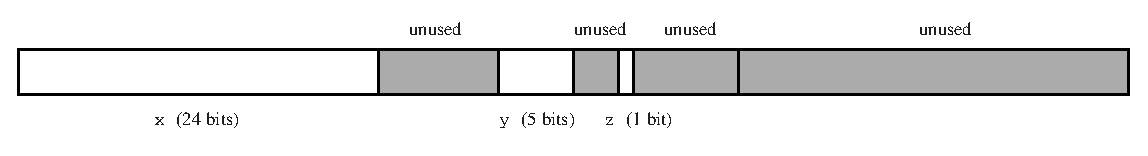
\includegraphics[scale=0.7]{Figures/standardAlignment.eps}\\
``Byte'' alignment byte-aligns the object and all fields:
\hfill\raisebox{-1ex}[0pt][0pt]{\parbox[t]{3in}{
\begin{samplecode}
class A \{\\
\>int x;  /* actual width 24 bits */\\
\>byte y; /* actual width 5 bits */\\
\>boolean z; /* actual width 1 bit */\\
\}\\
\end{samplecode}
}}\\
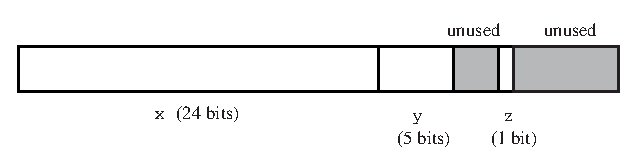
\includegraphics[scale=0.7]{Figures/byteAlignment.eps}\\
``Bit'' alignment requires no alignment of objects or fields:\\
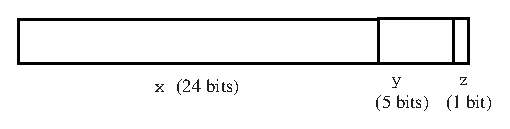
\includegraphics[scale=0.7]{Figures/bitAlignment.eps}\\
\hline
\end{tabular}
\caption{An example of different field packing scenarios.  The object
  header has been omitted for clarity.}
\label{fig:packing}
\end{figure*}

A typical Java implementation may waste large amounts of space by
aligning fields for the most efficient memory access.
Figure~\ref{fig:packing} illustrates how a class with an integer,
byte, and boolean field is typically laid out.  Our implementation
uses byte-packing to reduce the amount of wasted space in the object.
It is worth noting that the information provided by our bitwidth
analysis is sufficient to {\it bit}-pack the fields in the object,
when space is truely at a premium.  However, our investigation
indicates that the amount of space potentially gained by bit-packing 
is typically only a few percent.  Our implemented compiler uses byte
packing.

Some architectures penalize unaligned accesses to fields.  It is
worthwhile to {\it attempt} to align fields to their preferred
alignment while not allowing this to cause the object size to grow.
Further, there are often {\it forced} alignment constraints on
(for example) pointers.  Our Java runtime uses a conservative garbage
collector; its efficiency decreases markedly if pointers are not
word-aligned.

We have developed a simple byte-packing heuristic that achieves
tight packing of fields while respecting forced alignments.  Packing
proceeds recursively through superclasses, and returns a list of
free-space intervals available between the fields of the superclass.
The algorithm first places all {\it forced-alignment} fields in
the class, from largest to smallest.  The aim is for the
alignment-induced spaces left by the large fields to be fillable by
the following smaller fields.

When there are no more forced-alignment fields, we attempt to allocate
fields on their ``preferred'' alignment boundaries, largest first.
At this stage fields are not allowed to introduce an alignment gap at
the end of the object.  That is, if they cannot be placed flush
against the last field of the object and be on their preferred
alignment, they are skipped.

Finally, when there are no more preferred-alignments available, we
allocate the {\it smallest} available field, ignoring any preferred
alignment.  The aim is that the small fields will fill space and nudge
the end of the object out so that a larger field may be allocated on
its preferred alignment.  After each small field is allocated
unaligned, we try again to allocate fields on their preferred
boundaries.

This heuristic strategy has been observed to work well in practice,
and the penalties for occasionally placing an unaligned field have not
been observed to have a material adverse effect on performance (see
Section~\ref{sec:byte-pack}). 

% header optimizations.
% java-vs-byte-vs-bit packing.
% byte-packing strategy.
% garbage collection; dynamic methods.  conservative gc. ole aggeson's blah.
% efficiency of field virtualization.
% single-inheritance when splitting.
% efficiency of external hashtable
% distribution of mostly-constants.
% array allocation?
% pointer size improvements.
% parameter widening; reflection; interface to native code. stoplist

% header optimizations.
% pointer compression?

\subsection{External hashtable implementation}
\label{sec:extern-impl}
Close attention to the implementation of the hashtable used to
implement field and hash/lock externalization is
necessary to realize the gains possible in theory.  In order to
maximize space savings, it is necessary to utilize as little space
per field stored in the table as possible.  The overhead of
dynamically allocated buckets and the required {\it next} pointers
makes separate chaining impractical as an implementation technique
for all but fields with very few non-zero entries.  Open-addressing
implementations are preferable: in addition to the value being stored,
all that is necessary is a key value and the empty space required to
limit the load-factor.  A load factor of two-thirds and one-word keys
and values yield an average space consumption of three words per
field.  This implementation breaks even when the mostly-zero fields
identified are zero over 66\% of the time.  This break-even point is
compared to the profiling data to allow our field externalization
transformation to intelligently choose targetted fields.

Key-size reduction is an important component of the implementation:
a na{\"\i}ve approach
would combine a one-word reference to the virtual-container object and a
one-word field identifier for a two-word key.  The large key will
shift the break-even point up so that only fields which are 82\% zero
will profit.  Instead, we can offset the
object reference (up to the limit of its size) by small integers
to discriminate the externalized fields of the object, which yields
a single-word key.  This technique is
subject to object-size-dependent limits on the number
of class fields which may be externalized, but these have not been an
issue in practice.

Our implementation uses the garbage collector's object finalization
functionality to remove unneeded entries from the hashtable.  Care
must be taken, however, that the key value used in the hashtable
is not confused for an object pointer by a conservative garbage
collector.  Precise garbage-collection implementations need to
remember to add the values stored in the hashtable to the
collector's root set.

\section{Experimental Results}
\label{sec:results}

We have implemented all of the analyses and transformations described
in this paper in the MIT FLEX compiler infrastructure.%
\footnote{Available from {\tt http://flexc.lcs.mit.edu/}.} 
We measure the effectiveness
of our optimizations by compiling the SPECjvm98 benchmarks with 
this compiler, then measuring the resulting space savings and
performance.   All benchmarks were run on a dual-processor 900 MHz
Pentium III running Linux.

\subsection{Memory Savings}

To evaluate the effectiveness of our technique at reducing the
amount of memory required to execute the program, 
we first ran an instrumented version of each
application without any space optimizations. We used this
instrumented version to compute the total amount of data live on the
heap at any point during the execution.  
We then ran an instrumented version of our program after each stage of
optimization.
These versions enabled us to calculate the amount by which each 
technique reduced the size of the live heap data.

\begin{figure}
\includegraphics[scale=0.32,clip=true]{Figures/oopsla-ttllive.eps}
\caption{Reduction in the maximum live heap achieved with our
  transformations.}
\label{fig:live-heap}
\end{figure}

Figure~\ref{fig:live-heap} presents the total space savings numbers. This
figure contains a bar for each application, with the bar broken
down into categories that indicate the percentage of live data from 
the original unoptimized execution that we were able to eliminate
with each optimization. The black section of each bar indicates the
amount of live heap data remaining after all optimizations. 
We obtain as much as 40\% reduction in live data on the {\tt
  213\_javac} benchmark, with almost all of this coming from our
bitwidth-driven field reductions and static specialization.  In fact
we obtain more than 15\% reduction on all of the ``object-oriented''
benchmarks.  The {\tt 201\_compress} benchmark allocates a small
number of very large arrays, limiting the optimization opportunities
discoverable by our analysis.  Likewise, the {\tt 205\_raytrace} and
{\tt 227\_mtrt} benchmarks make heavy use of floating-point numbers.
However, these raytracing benchmarks {\it do} allocate a large number
of small arrays to represent vectors and matrices, and so our header
optimizations still allow us to reduce the maximum live data size by
over 20\%.

We also used an instrumented executable to determine the total amount
of memory allocated during the entire execution of the program, in
both the optimized and unoptimized versions.  Reducing this total
allocation reduces the load on the garbage collector.
Figure~\ref{fig:total-alloc} presents the space savings according to this
metric.  By comparing to the previous figure, you will notice that
long-lived objects apparently provide us with more opportunities to
optimize.

\begin{figure}
\includegraphics[scale=0.32,clip=true]{Figures/oopsla-ttlalloc.eps}
\caption{Cumulative reduction in dynamic allocation achieved with
  our transformations.}
\label{fig:total-alloc}
\end{figure}

\subsection{Objects Versus Arrays}

The majority of our optimizations are designed to optimize
object fields rather than arrays. For context, we present numbers 
that characterize the reductions in total allocation for objects only,
rather than for both objects and arrays. Figure~\ref{fig:non-array}
presents space savings numbers for objects alone, omitting
any storage required for arrays.  The difference is explained by
Figure~\ref{fig:object-array-pointer}, which shows how the total
program allocation for each benchmark is broken down into array and
object allocations.  The space required for pointer fields, which our
integer bitwidth analysis can not optimize, are further broken out of
the object allocations.
The reason for our poor performance on {\tt
  201\_compress} is now obvious.  Note that {\tt 222\_mpegaudio}
allocates so much less memory than the other benchmarks that its bar
is barely visible.  Arrays account for 79\% of {\tt mpegaudio}'s total
allocations.

\begin{figure}
\includegraphics[scale=0.32,clip=true]{Figures/oopsla-objalloc.eps}
\caption{Reduction in non-array dynamic allocation achieved with
  our transformations.}
\label{fig:non-array}
\end{figure}

\begin{figure}
\includegraphics[scale=0.32,clip=true]{Figures/spec-space.eps}
\caption{Total allocation in spec benchmarks.}
\label{fig:object-array-pointer}
\end{figure}

\subsection{Execution Times} 
\label{sec:byte-pack}

We next evaluate the execution time impact of applying our space
optimizations. Figure~\ref{fig:performance} presents the normalized execution 
times of each application after the application of our sequence
of optimizations. These numbers show that the first several
optimizations (claz compression, field reduction, and byte packing)
typically reduce the execution times, while the
remainder (static specialization, field externalization, and  hash/lock
externalization) generate modest increases in the execution times. 
Static specialization's virtualization of fields is responsible for
its slowdown; it is likely that an optimized speculatively-inlined
implementation of the field accessors which it adds to the program
would improve its performance.  Field externalization (including
hash/lock externalization) causes the expected penalty for hashtable
lookup; note that synchronization elimination would greatly reduce the
cost of hash/lock externalization.

\begin{figure}
\includegraphics[scale=0.32,clip=true]{Figures/oopsla-speed.eps}
\caption{Runtime performance of space optimizations.}
\label{fig:performance}
\end{figure}

% distribution of mostly-N fields?

\section{Related work}

Many researchers have focused on the problem of reducing the amount of
header space required to represent Java
locks~\cite{bacon98,OK99,ADGKRW99}. The basic issue is that the vast
majority of programs do not use the lock associated with every object
in its full generality, so it is possible to develop improved
algorithms optimized for the common case rather than the most general
case. The basic idea is to represent the lock with the minimum amount
of state (typically a bit) required to support the common usage
pattern of a thread first acquiring, then releasing the lock in the
object and to back off to a more elaborate scheme only when the thread
exhibits a more complex pattern such as nested lock acquires. The
primary focus has been on improving performance rather than on
reducing space; however, many of the algorithms also eliminate the
need to store the complicated locking objects required to support the
most general lock usage pattern possible in a Java program. These
techniques typically reduce the lock space overhead to 24 header bits
\cite{bacon98}.

Research in escape analysis and related analyses can enable the
compiler to find objects whose locks are never 
acquired~\cite{ACSE99,BH99,whaley99,CGSSM99,Ruf00:PLDI00,salcianu01}.
This information can enable the compiler to remove the space
reserved for synchronization support in these objects. 
Our hash/lock removal algorithm uses a totally dynamic approach
based on our field externalization mechanism. 

Several researchers have used bitwidth analysis to reduce the size
of the generated circuits for compilers that generate hardware
implementations of programs written in C or similar programming 
languages~\cite{ananian:siliconc,RR00:PLDI00,stephenson00,BGSW00}.

Dieckmann and Hoelzle have performed an in-depth analysis of the
memory allocation behavior of Java programs~\cite{DH99}. Although 
space is not their primary focus, their study does quantify 
the space overhead associated the use of a two-word header
and of 8-byte alignment. In general, our measurements of the 
memory system behavior of Java programs broadly agree with their
measurements. 

Sweeny and Tip \cite{SweeneyTip98DeadDataMembers} did a study of dead
members of C++ programs, which is similar to the unread field
elimination done by our bitwidth analysis.  However, they
fail to identify {\it constant} members, which our SCC-based algorithm
does easily.  Further, our results show that unread and constant field
elimination is very dependent on the coding style of a particular
application.  The collection of techniques we have presented here
gives much more consistent savings over a wide range of benchmarks.

%Aggarwal and Randall \cite{aggarwal01} described a array bounds check
%removal method using {\it related fields}.  This work attempted to
%discover fields, such as {\tt Vector.size}, which are guaranteed to be
%less than or equal to the length of some array, for example, the
%backing array stored in {\tt Vector.data}.  Tests against the related
%field could then provide information about bounds checks on accesses
%to the array.  A similar technique could be used in this work to
%extend the utility of bitwidth information discovered on related fields.


\section{Conclusions}

We have presented a set of techniques for reducing the memory
consumption of object-oriented programs.  Our techniques include
program analyses to detect unused, constant, or overly-wide fields,
and transformations to eliminate fields with common default values
or usage patterns.  These techniques apply equally well to
field implicit in the runtime's object header, and can reduce the
maximum heap required for a program by as much as 40\%. 
Our experimental results from our fully-implemented system validate the
opportunity for space savings on typical object oriented programs.

\bibliography{harpoon}

%\appendix
%\input{pldi02-appendix}
\end{document}
